% Author: Dominic van der Zypen
% Edited using vi

\documentclass[11pt,reqno]{amsart}

\usepackage{amsmath,amssymb,amsthm}
\usepackage{hyperref}
\usepackage{geometry}
\geometry{margin=1.25in}

% --- TikZ Packages ---
\usepackage{tikz}
\usetikzlibrary{positioning, arrows.meta}

% --- Theorem Styles ---
\newtheorem{theorem}{Theorem}[section]
\newtheorem{lemma}[theorem]{Lemma}
\newtheorem{proposition}[theorem]{Proposition}
\newtheorem{conjecture}[theorem]{Conjecture}
\newtheorem{problem}[theorem]{Problem}

\theoremstyle{definition}
\newtheorem{definition}[theorem]{Definition}
\newtheorem{example}[theorem]{Example}
\newtheorem{remark}[theorem]{Remark}

% --- Custom Commands ---
\newcommand{\F}{\mathbb{F}_2}
\newcommand{\Maj}{\mathrm{Maj}}

\title{Majority-based Feedback Shift Registers}

\author{Dominic van der Zypen}
\email{dominic.zypen@gmail.com} % Replace with your actual email

\begin{document}

\parindent = 0mm
\parskip = 2mm

\begin{abstract}
We introduce and explore \emph{Majority-based Feedback Shift Registers} (MFSRs), 
a class of non-linear feedback shift registers where the linear XOR 
feedback function of traditional LFSRs is replaced by a symmetric majority 
voting mechanism over selected tap positions. While linear feedback 
shift registers over $\F$ benefit from the algebraic theory of 
primitive polynomials to guarantee maximal cycle lengths of $2^n - 1$, 
majority feedback introduces strong non-linear dynamics that break 
vector-space symmetries. We formalize the transition dynamics of 
MFSRs, report preliminary numerical observations on state-space fragmentation 
and cycle lengths, and highlight open problems regarding the maximum 
attainable period and structural tap configurations.
\end{abstract}

\maketitle

%------------------------------------
\section{Introduction}

Linear Feedback Shift Registers (LFSRs) are fundamental building blocks in stream 
cipher design, pseudo-random number generation, and hardware 
testing \cite{Golomb1982, Rueppel1986, Menezes1996}. An $n$-bit LFSR 
updates its state by shifting bits and computing a new 
feedback bit via a linear combination (addition modulo 2) of chosen tap positions:
\[
s_{t+n} = \sum_{i=1}^{n} c_i s_{t+n-i} \pmod 2, \quad c_i \in \F.
\]

\begin{figure}[htbp]
\centering
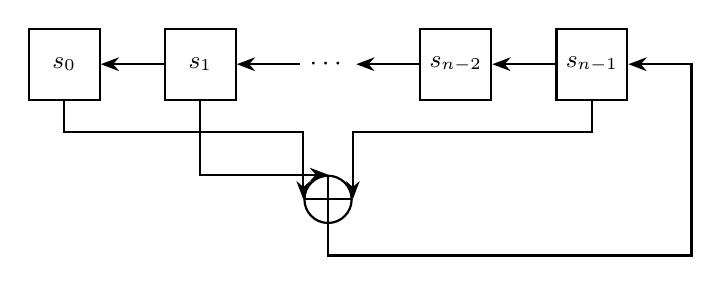
\begin{tikzpicture}[
    box/.style={rectangle, draw, thick, minimum width=0.9cm, minimum height=0.9cm, align=center, font=\small},
    xor/.style={circle, draw, thick, minimum size=0.6cm, inner sep=0pt,
        path picture={
            \draw[thick] (path picture bounding box.south) -- (path picture bounding box.north);
            \draw[thick] (path picture bounding box.west) -- (path picture bounding box.east);
        }
    },
    >=Stealth,
    node distance=0.8cm
]
    % Registers
    \node[box] (s0) {$s_0$};
    \node[box, right=of s0] (s1) {$s_1$};
    \node[right=of s1] (dots) {$\cdots$};
    \node[box, right=of dots] (sn2) {$s_{n-2}$};
    \node[box, right=of sn2] (sn1) {$s_{n-1}$};

    % Shift arrows (leftward shift)
    \draw[->, thick] (s1.west) -- (s0.east);
    \draw[->, thick] (dots) -- (s1.east);
    \draw[->, thick] (sn2.west) -- (dots);
    \draw[->, thick] (sn1.west) -- (sn2.east);

    % XOR gate for feedback
    \node[xor, below=1.2cm of dots] (xor) {};

    % Tap connections from s_0, s_1, s_{n-1} to XOR
    \draw[->, thick] (s0.south) |- ([yshift=-0.4cm]s0.south) -| (xor.west);
    \draw[->, thick] (s1.south) |- (xor.north);
    \draw[->, thick] (sn1.south) |- ([yshift=-0.4cm]sn1.south) -| (xor.east);

    % Feedback path from XOR to input of s_{n-1}
    \draw[->, thick] (xor.south) -- ++(0,-0.4) -| ([xshift=0.8cm]sn1.east) -- (sn1.east);

\end{tikzpicture}
\caption{An $n$-bit Linear Feedback Shift Register with 3 taps ($s_0, s_1, s_{n-1}$).}
\label{fig:lfsr}
\end{figure}

When the feedback polynomial 
$f(x) = 1 + \sum_{i=1}^n c_i x^i$ is primitive 
over $\F$, the state sequence achieves the maximum possible period of 
$2^n - 1$ for non-zero initial states \cite{Golomb1982}.

In this note, we study a natural non-linear modification: replacing the 
linear parity check (XOR) with a majority threshold gate. 

%------------------------------------
\section{Formal Definition}
Let $\mathcal{S}_t = (s_{t, 0}, s_{t, 1}, \dots, s_{t, n-1}) \in \{0, 1\}^n$ 
denote the state of an $n$-bit shift register at clock cycle $t$.

\begin{definition}[Majority Function]
For an odd integer $k \ge 3$, the Boolean majority 
function $\Maj \colon \{0, 1\}^k \to \{0, 1\}$ is defined by
\[
\Maj(x_1, x_2, \dots, x_k) = 
\begin{cases} 
1 & \text{if } \sum_{i=1}^k x_i \ge \frac{k+1}{2}, \\
0 & \text{otherwise.}
\end{cases}
\]
\end{definition}

\begin{definition}[Majority-based Feedback Shift Register]
Let $T = \{i_1, i_2, \dots, i_k\} \subseteq \{0, 1, \dots, n-1\}$ 
be a set of $k$ distinct tap positions, where $k$ is odd. 
The transition rule of the corresponding 
{\em Majority-based Feedback Shift Register} (MFSR) updates 
state $\mathcal{S}_t$ to $\mathcal{S}_{t+1}$ according to:
\[
s_{t+1, j} = 
\begin{cases}
s_{t, j+1} & \text{for } 0 \le j < n-1, \\
\Maj(s_{t, i_1}, s_{t, i_2}, \dots, s_{t, i_k}) & \text{for } j = n-1.
\end{cases}
\]
\end{definition}

\begin{figure}[htbp]
\centering
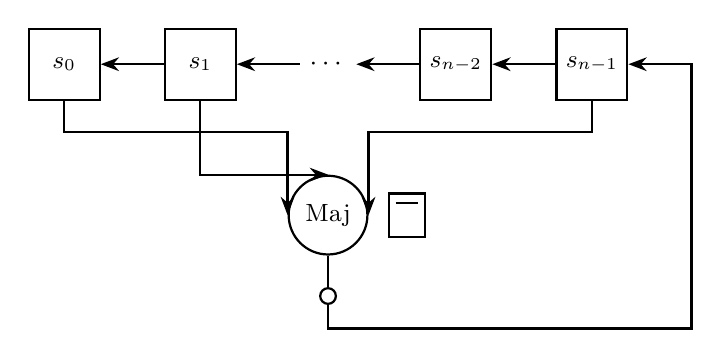
\begin{tikzpicture}[
    box/.style={rectangle, draw, thick, minimum width=0.9cm, minimum height=0.9cm, align=center, font=\small},
    maj/.style={circle, draw, thick, minimum size=1.0cm, inner sep=0pt, align=center, font=\small},
    inverter/.style={circle, draw, thick, inner sep=2pt, fill=white},
    votingbox/.style={rectangle, draw, thick, minimum width=0.45cm, minimum height=0.55cm, inner sep=1pt, fill=white,
        path picture={
            \draw[thick] (path picture bounding box.north west) ++(0.08cm, -0.12cm) -- ++(0.29cm, 0);
        }
    },
    >=Stealth,
    node distance=0.8cm
]
    % Registers
    \node[box] (s0) {$s_0$};
    \node[box, right=of s0] (s1) {$s_1$};
    \node[right=of s1] (dots) {$\cdots$};
    \node[box, right=of dots] (sn2) {$s_{n-2}$};
    \node[box, right=of sn2] (sn1) {$s_{n-1}$};

    % Shift arrows (leftward shift)
    \draw[->, thick] (s1.west) -- (s0.east);
    \draw[->, thick] (dots) -- (s1.east);
    \draw[->, thick] (sn2.west) -- (dots);
    \draw[->, thick] (sn1.west) -- (sn2.east);

    % Majority gate and voting box for feedback
    \node[maj, below=1.2cm of dots] (maj) {$\mathrm{Maj}$};
    \node[votingbox, right=0.25cm of maj] (vbox) {};

    % Tap connections from s_0, s_1, s_{n-1} to Maj
    \draw[->, thick] (s0.south) |- ([yshift=-0.4cm]s0.south) -| (maj.west);
    \draw[->, thick] (s1.south) |- (maj.north);
    \draw[->, thick] (sn1.south) |- ([yshift=-0.4cm]sn1.south) -| (maj.east);

    % Feedback path with negation from Maj to input of s_{n-1}
    \draw[thick] (maj.south) -- ++(0,-0.4);
    \node[inverter, below=0.4cm of maj.south] (inv) {};
    \draw[->, thick] (inv.south) -- ++(0,-0.3) -| ([xshift=0.8cm]sn1.east) -- (sn1.east);

\end{tikzpicture}
\caption{An $n$-bit Majority-based Feedback Shift Register (MFSR) with 
3 taps ($s_0, s_1, s_{n-1}$). The majority voting function 
is symbolized by a little ballot box, and the small circle $\circ$
	denotes feedback negation.}
\label{fig:mfsr}
\end{figure}

\begin{remark}[Efficient Bitwise Implementation]
For software implementations, the evaluation of the majority 
feedback can be streamlined using native bitwise arithmetic and 
population count ({\tt popcount}) operations. Specifically, 
after masking the state with the tap set $T$, one can compute the 
{\tt popcount}) of active taps. Since $|T|$ is odd,
the majority condition checking whether 1s account for more than 
half of the taps just means comparing $|T|$ against 
	$(\text{popcount} \ll 1)$ without floating-point divisions or conditionals.
\end{remark}


%------------------------------------
\section{State-Space Dynamics and Non-Linearity}

Because the majority operator is non-linear, the state evolution 
operator $F \colon \{0, 1\}^n \to \{0, 1\}^n$ does not 
preserve linear combinations, meaning that {\sl in general} we have
\[
F(\alpha \cdot \mathcal{S}_A + \beta \cdot \mathcal{S}_B) \neq \alpha F(\mathcal{S}_A) + \beta F(\mathcal{S}_B).
\]
Consequently, the state space $\{0, 1\}^n$ does not partition into 
neat linear cycles. Instead, empirical observations reveal:
\begin{enumerate}
    \item {\bf Attractors and Short Cycles:} For many tap choices $T$, large 
	   portions of the state space collapse into short periodic orbits
	or fixed points (such as the all-zero or all-one states).
    \item {\bf Transient States:} Unlike invertible linear shift registers 
	    (where every state lies on a cycle), majority feedback is 
	non-invertible, creating state-space trees leading to cycle basins.
\end{enumerate}

%------------------------------------
\section{Open Problems and Conjectures}

The main challenge in studying MFSRs lies in overcoming the 
absence of Galois field arithmetic to bound cycle lengths.

\begin{problem}[Maximal Cycle Bounds]
Given register length $n$, what is the upper bound on the period 
	$P(n, T)$ of a cycle generated by an $n$-bit MFSR with tap set $T$ 
	(where $|T|$ is odd)?
\end{problem}

\begin{conjecture}[Existence of Long Cycles]
For every register length $n$, there exists a tap set $T$ having odd cardinality,
	such that the maximum cycle length satisfies:
\[
P_{\max}(n) \approx 2^n(1 - o(1)).
\]
\end{conjecture}

\begin{problem}[Tap Selection Principles]
Are there systematic or algebraic criteria for choosing tap sets $T$ that prevent premature collapse into short cycle attractors?
\end{problem}

%------------------------------------
{\bf Code and Implementation.}
Source code in C for simulating $n$-bit MFSR dynamics and analyzing 
state-space graph structures is available 
at \url{https://github.com/dominiczypen/Majority_Feedback_Shift_Register}.

\vspace*{3mm}

%------------------------------------
{\bf AI disclaimer.} AI has been used solely for drawing the
figures \ref{fig:lfsr} and \ref{fig:mfsr}.


\begin{thebibliography}{99}

\bibitem{Golomb1982}
S.~W. Golomb, \emph{Shift Register Sequences}, rev. ed., Aegean Park Press, 1982.

\bibitem{Menezes1996}
A.~J. Menezes, P.~C. van Oorschot, and S.~A. Vanstone, \emph{Handbook of Applied Cryptography}, CRC Press, 1996.

\bibitem{Rueppel1986}
R.~A. Rueppel, \emph{Analysis and Design of Stream Ciphers}, Springer-Verlag, 1986.

\end{thebibliography}

\end{document}